\chapter{Marco te\'orico}\label{capit:cap2}
\vspace{-2.0325ex}%
\noindent
\rule{\textwidth}{0.5pt}
\vspace{-5.5ex}% 
\newcommand{\pushline}{\Indp}% Indent puede ir o no :p

En este capítulo se definen una serie de conceptos importantes del área de procesamiento de imágenes y reconocimiento de patrones, estas definiciones son importantes para la comprensión del tema.


%--------------------------------------------------------------------------------------------------------------------------------


\section{Gestos}\label{sec:2Gestos}
Los gestos \citep{Mitra2007} son movimientos del cuerpo expresivos y significativos que involucran dedos, manos, brazos, cabeza, cara o cuerpo con la intención de transmitir información relevante o interactuar con el ambiente. \\
De acuerdo con la literatura \citep{Mitra2007} los gestos con las manos se clasifican en estáticos y dinámicos, los primeros están definidos como la posición y orientación de la mano en el espacio manteniendo esta pose durante cierto tiempo, por ejemplo para hacer una se\~nal de aventón, a diferencia de los gestos dinámicos donde hay movimiento de la pose, un ejemplo  es cuando mueves la mano en se\~nal de adiós. 


%--------------------------------------------------------------------------------------------------------------------------------

\section{Reconocimiento de gestos con la manos}\label{sec:2ReconocimientoGestos}   

El reconocimiento de gestos con las manos consiste no solo en el seguimiento del movimiento de la o las manos realizados por un emisor, también en la interpretación de este movimiento por un receptor, \citep{Mitra2007}, \citep{Murthy2009}.\\
De aquí en adelante entiéndase el término gestos con las manos, como gestos.   

En el capítulo \ref{capit:cap1} sección \ref{sec:ReconocimientoGestos}, se explicó que existen dos modelos utilizados para el reconocimiento de gestos dependiendo del dispositivo de captura, los basados en contacto y en la visión.\\
Los métodos basados en la visión realizan la representación del gesto con diferentes técnicas las cuales se separan en dos categorías \citep{Rautaray2012}: basados en apariencia y basados en un modelo 3D. Los basados en un modelos 3D convierten los datos en entrada en una forma espacial y los basados en apariencia utilizan los datos 2D de la imagen de entrada.      

De acuerdo con la literatura el proceso de reconocimiento de gestos basados en la visión se dividen en tres \citep{Rautaray2012} fases que son: detección; extracción de características o seguimiento, dependiendo si los gestos son dinámicos; por último el reconocimiento del gesto. Otros autores \citep{Hasan2012} incluyen la etapa de adquisición de datos. Las etapas se abordaran en la sección siguiente. 


\subsection{Etapas del reconocimiento}\label{subsec:EtapasReconocimiento}  
En la sección se abordaron las estas etapas del reconocimiento y se mencionan los principales algoritmos utilizados en cada una de estas etapas. El diagrama de la figura \ref{fig:HGR} muestra las etapas del reconocimiento.  

\begin{figure}[h!]
\begin{center}
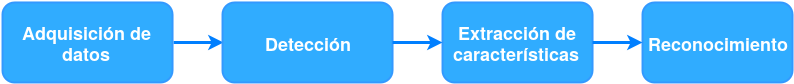
\includegraphics[scale=.6]{./Figures/HGR.png}
\end{center}
\caption{El diagrama ejemplifica el procedimiento del reconocimiento de gestos.}
\label{fig:HGR}
\end{figure}

El proceso de reconocimiento varia un poco dependiendo del tipo de gesto, si es estático o dinámico. Por ejemplo el diagrama \ref{fig:HGR} ejemplifica perfectamente el proceso de reconocimiento de un gestos estático, para los gestos dinámicos se necesita una fase extra, el seguimiento el cual se realizada una vez detectada la mano, esta puede estar englobada en la fase de extracción de características o viceversa. 

\subsubsection{Adquisición de datos}\label{sssec:EtapaAdquisicion}

Es la primera etapa del reconocimiento en la cual los datos son capturados. En el modelo basado en la visión se utilizan cámaras como: 

La información obtenida es representado como imágenes. 

\subsubsection{Detección}\label{sssec:EtapaDeteccion}

En esta etapa se localiza y segmenta la mano del fondo de la imagen para obtener las características necesarias para identificar el gesto.\\
Existen distintos métodos para obtener dichas características como la de color de la piel, forma, movimiento, entre otras que generalmente son combinaciones de alguna de estas, para obtener un mejor resultado. Enseguida se describe brevemente cada una de estas.  
\begin{itemize}
\item Color de la piel: Se basa principalmente en escoger un espacio del color, es una organización de colores especifica; como; RGB (rojo, verde, azul), RG (rojo, green), YCrCb (brillo, la diferencia entre el brillo y el rojo, la diferencia entre el brillo y el azul), etc. La desventaja es que si es color de la piel es similar al fondo, la segmentación no es buena, la forma de corregir esta segmentación es suponiendo que el fondo no se mueve con respecto a la cámara.
\item Forma: Extrae el contorno de las imágenes, si se realiza correctamente se obtiene el contorno de la mano. Aunque si se toman las yemas de los dedos como características, estas pueden ser ocluidas por el resto de la mano, una posible solución es usar más de una cámara.  
\item Valor de p\'ixeles: Usar imágenes en tonos de gris para detectar la mano en base a la apariencia y textura, esto se logra entrenando un clasificador con un conjunto de imágenes.
\item Modelo 3D: Depende de cual modelo se utilice, son las características de la mano requeridas. 
\item Movimiento: Generalmente esta se usa con otras formas de detección ya que para utilizarse por sí sola hay que asumir que el único objeto con movimiento es la mano.
\end{itemize} 

La segmentación es la partición o separación de la imagen en regiones representativas, es decir separar la mano del fondo de la imagen. Existen diversos métodos para llevar acabo la segmentación de la mano los cuales se clasifican en cuatro clases, basados en pixeles los cuales hacen la separación usando el valor del nivel de gris en la imagen; en el borde estos métodos utilizan los pixeles que representan las orillas del objeto y encuentran el correspondiente contorno; en regiones los cuales van agrupando vecindarios de la imagen de acuerdo a ciertas propiedades; por ultimo la segmentación basada en un modelo la cual hacen uso de algún modelo definido, estos requieren imágenes de entrenamiento para representar la probabilidad de las muestras registradas y finalmente hace inferencias en la imagen \citep{Ibraheem2013}.
Enseguida se presentan algunas técnicas para realizar la segmentación.
\begin{itemize}
\item Color de la piel: Se basa principalmente en escoger un espacio del color, es una organización de colores especifica; como; RGB (rojo, verde, azul), RG (rojo, green), YCrCb (brillo, la diferencia entre el brillo y el rojo, la diferencia entre el brillo y el azul), etc. La desventaja es que si es color de la piel es similar al fondo, la segmentación no es buena, la forma de corregir esta segmentación es suponiendo que el fondo no se mueve con respecto a la cámara.
\end{itemize}

\subsubsection{Extracción de características y seguimiento}\label{sssec:EtapaSeguimiento}  

La extracción de características consiste en obtener ciertas entradas medibles de la imagen de la mano, generalmente segmentada, las cuales son utilizadas para reconocer el gesto realizado, \citep{Premaratne2013}, \citep{Nayakwadi2014}.\\
Existen dos tipos de características geométricas tales como: las yemas de los dedos, la dirección de los dedos, el contorno de la mano y entre otras características; y las características no geométricas como el color, siluetas y texturas. \citep{Murthy2009}. 

Enseguida se mencionan algunas de los métodos para la obtención de características \citep{Premaratne2013}. 
\begin{itemize}
\item Descriptores de Fourier los cuales describen formas en la imagen, haciendo uso de la serie de Fourier. Estas características son invariantes a escala.
\item Descriptores de Contorno nos dan el contorno  o el límite del objeto con invariancia a traslación, escala  y reflexión.     
\item Características descritas por histogramas. Histogramas de gradientes orientados (HOG) es un descriptor de características. Se trata de contar la orientación de los gradientes en cierta porción de la imagen.  
\end{itemize}



Consiste en localizar la mano en cada cuadro (imagen). Se lleva acabo usando los métodos de detección si estos son lo suficientemente rápidos para detectar la mano cuadro por cuadro. Se explica brevemente los métodos para llevar a cabo el seguimiento. 
\begin{itemize}
	\item Basado en plantillas: Este se divide en dos categorías (Características basadas en su correlación y basadas en contorno), que son similares a los métodos de detección, aunque supone que las imágenes son adquiridas con la frecuencia suficiente para llevar acabo el seguimiento. Características basadas en su correlación, sigue las características a través de cada cuadro, se asume que las características aparecen en mismo vecindario. Basadas en contorno, se basa en contornos deformables, consiste en colocar el contorno cerca de la región de interés e ir deformando este hasta encontrar la mano. 
	\item Estimación óptima: Consiste en usar filtros Kalman, un conjunto de ecuaciones matemáticas que proporciona una forma  computacionalmente eficiente y recursiva de estimar el estado de un proceso, de una manera que minimiza la media de un error cuadrático, el filtro soporta estimaciones del pasado, presente y futuros estados, y puede hacerlo incluso cuando la naturaleza precisa del modelo del sistema es desconocida;  para hacer la detección de características en la trayectoria. 
	\item Filtrado de partículas: Un método de estimación del estado de un sistema que cambia a lo largo del tiempo, este se compone de un conjunto de partículas (muestras) con pesos asignados, las partículas son estados posibles del proceso. Es utilizado cuando no se distingue bien la mano en la imagen. Por medio de partículas localiza la mano la desventaja es que se requieren demasiadas partículas, y el seguimiento se vuelve imposible. 
	\item Camshift: Busca el objetivo, en este caso la mano, encuentra el patrón de distribución mas similar en una secuencia de imágenes, la distribución puede basada en el color. 
\end{itemize}

\subsubsection{Reconocimiento}\label{sssec:EtapaReconocimiento}

Es reconocimiento es la etapa final de este proceso, la cual consiste en identificar el gesto utilizando alguna técnica de clasificación.\\
El método de clasificación a utilizar se elige dependiendo del tipo de gesto a reconocer, por ejemplo para los gestos estáticos se realiza el empatamiento del gesto con una plantilla previamente calculada; en los gestos dinámicos generalmente  se usan algoritmos de aprendizaje de máquina. Aunque los más utilizados son los algoritmos de redes neuronales, maquina de soporte vectorial y modelo oculto de Markov\\ 
A continuación se encuentran los principales métodos para llevar acabo el reconocimiento del gestos \citep{Rautaray2012}. 
\begin{itemize}
	\item K-medias: Es un método de agrupamiento el cual consiste en determinar los $k$ puntos llamados centros para minimizar el error de agrupamiento, que es la suma de las distancias de todo los puntos al centro de cada grupo. El algoritmo empieza localizando aleatoriamente $k$ grupos en el espacio espectral. Cada p\'ixel en la imagen de entrada es entonces asignadas al centro del grupo mas cercano  
	\item Desplazamiento de medias: Es un método iterativo que encuentra el máximo en una función de densidad dada una muestra estadística de los datos.
	\item Máquinas de soporte vectorial: Consiste en un mapeo no lineal de los datos de entrada a un espacio de dimensi\'on m\'as grande, donde los datos pueden ser separados de forma lineal.  
	\item Modelo oculto de Markov: Es definido como un conjunto de estados donde, un estado inicial, un conjunto de símbolos de salida y un conjunto de estados de transición. En el reconocimiento de gestos se puede caracterizar a    los estados como un conjunto de las posiciones de la mano; las  transiciones de los estados como la probabilidad de transición de cierta posición de la mano a otra; el símbolo de salida como una postura especifica y la secuencia de los símbolos de salida como  el gesto de la mano.   
	\item Redes neuronales con retraso: Son una clase de redes neuronales artificiales que se enfocan en datos continuos, haciendo que el sistema sea adaptable para redes en linea y les da ventajas sobre aplicaciones en tiempo real. 
\end{itemize}  


%--------------------------------------------------------------------------------------------------------------------------------

\section{Imagen}\label{ImagenDef} 

Una imagen se puede definir como una función bidimensional, $S(x,y)$ donde $x$, $y$ representan las coordenadas en el plano y el valor de la función es la intensidad o nivel de gris en el punto $(x,y)$. 
Si el valor de la función y los puntos de la imagen son finitos, esta es una imagen digital, la cual se puede representar en una matriz donde cada valor o pixel es el nivel de gris de la imagen \ref{fig:image}, y los indices de esta indican la posición, \citep{Gonzalez2002}. 

\begin{figure}[h!]
\begin{center}
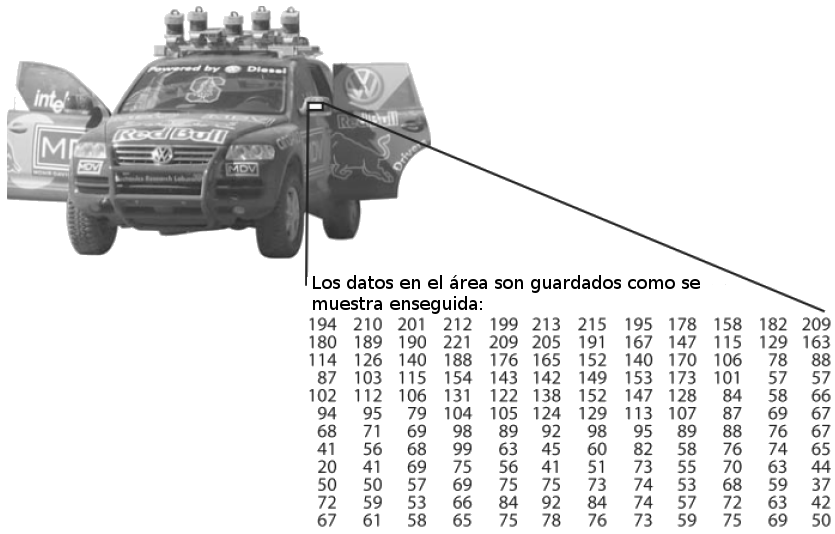
\includegraphics[scale=.50]{./Figures/image.png}
\end{center}
\caption{Representación de un imagen digital. Recuperada de \citep{Shin2013}}
\label{fig:image}
\end{figure}


%--------------------------------------------------------------------------------------------------------------------------------


%\section{Ruido}\label{RuidoImage}



%--------------------------------------------------------------------------------------------------------------------------------

\section{Obstrucción}\label{OclusionDef} 

Se puede definir una obstrucción como discontinuidades del movimiento y profundidad que se es percibida por un observador que se encuentra en movimiento en un ambiente estático.\\
Los puntos de obstrucción en una imagen o cuadro son pixeles que aparecen o desaparecen en dos cuadros consecutivos, estos son llamados puntos de obstrucción o punto de no obstrucción, \citep{Silva2001}.  

Existen tres tipos distintos de obstrucción la cuales depende de la forma en que es causada. Estas son: obstrucción por el mismo objeto, entre objetos y por el fondo. La obstrucción por el mismo objeto se presenta cuando parte del objeto obstruye a otra. La obstrucción entre objetos es cuando dos objetos que se siguen se obstruyen entre ellos mismos. La obstrucción por el fondo es cuando parte del fondo obstruye al objeto que se sigue, \citep{YilmazA.JavedO.andShah2006}


%-------------------------------------------------------------------------------------------------------------------------------- 


\section{Métricas de desempeño}\label{Metricas}

Existen diversos métodos para medir el rendimiento de un algoritmo de clasificación, una manera de representarlo es mediante una matriz de confusión. 

Considerando una clasificación de solo dos clases. Cada instancia es mapeada a un elemento del conjunto de etiquetas (positiva o negativa). El clasificador se encarga de mapear las instancias a las clases existentes, indicando la clase a a la que pertenece la instancia.\\
El resultado de clasificación de alguna instancia puede resultar en cuatro posibles estados. Si la instancia es positiva y la clasificación es positiva, es un verdadero positivo; si la clasificación es negativa es un falso negativo. Si la instancia es negativa y la clasificación es negativa, es un verdadero negativo; si la clasificación es positiva, es un falso positivo. \\ 
Dado un clasificador y un conjunto de instancias, una matriz de confusión de $2 \times 2$, como la que se muestra en la figura \ref{fig:Matrix} , puede ser construida por el resultado del conjunto de instancias.   
\begin{figure}[h!]
\begin{center}
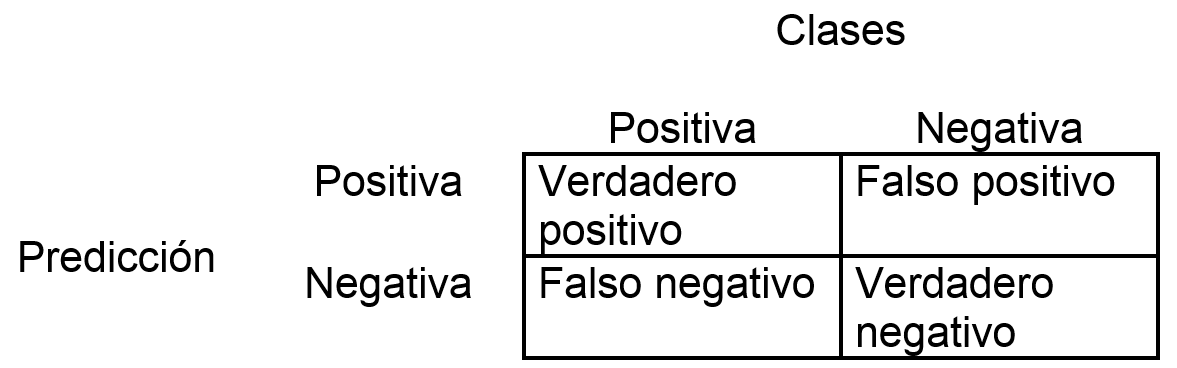
\includegraphics[scale=.4]{./Figures/MatrixConfusion.png}
\end{center}
\caption{La siguiente imagen representa matriz de confusión, de un problema de clasificación de dos clases.}
\label{fig:Matrix}
\end{figure}
Los valores de la diaginal de la matriz de confusion representan las predicciones correctas, y los valores fuera de la diagonal representan los errores.

Distintas métricas de desempeño pueden ser calculadas gracias a esta matriz.\\ 
La tasa de precision del clasificador puede ser calculado como: 
\begin{equation}
Presicion = \frac{Verdaderos \quad positivos}{Verdaderos \quad positivos + Falsos \quad positivos}
\end{equation}
La tasa de exactitud del clasificador puede ser calculado como: 
\begin{equation}
Exactitud = \frac{Verdaderos \quad positivos + Verdaderos \quad negativos}{Total \quad de \quad positivos + Total \quad de \quad negativos}
\end{equation}
La tasa de verdaderos positivos $Tp$, del clasificador puede ser calculada como: 
\begin{equation}
Tp \approx \frac{Positivos \quad clasificados \quad correctamente}{Total \quad de \quad  positivos}
\end{equation} 
La tasa de falsos positivos $Fp$, del clasificador puede ser calculada como: 
\begin{equation}
Fp \approx \frac{Negativos \quad clasificados \quad correctamente}{Total \quad de \quad negativos}
\end{equation}






\newpage
%%=====================================================
